\documentclass[conference]{IEEEtran}
\usepackage{graphicx,cite,bm,psfrag,amsmath,enumitem}
\def\mmax{\mathop{\mbox{\scriptsize max}}}
\def\argmin{\mathop{\mbox{arg\,min}}}
\def\argmax{\mathop{\mbox{arg\,max}}}
\newcommand{\defequal}{\stackrel{\mathrm{def}}{=}}
\renewcommand{\vec}[1]{{\ensuremath{\boldsymbol{#1}}}}
\newcommand{\popt}{\ensuremath{P^{(K)}_{opt}}}
\IEEEoverridecommandlockouts
\pagestyle{plain}
\usepackage{amsfonts}
\usepackage{algorithm, algorithmic}
\renewcommand{\algorithmicrequire}{ \textbf{Initialization:}} %Use Input in the format of Algorithm
\renewcommand{\algorithmicensure}{ \textbf{Procedures:}} %UseOutput in the format of Algorithm
% correct bad hyphenation here
%\hyphenation{op-tical net-works semi-conduc-tor}
\usepackage{CJK}
\usepackage{color}
\usepackage{url}
\usepackage{geometry}
\geometry{left=0.5in, right=0.5in, top=0.75in, bottom=0.75in}

\begin{document}
\title{Cluster-by-Cluster Block Diagonal Digital Precoding for Multi-User MIMO Downlink Transmissions}
\author{\IEEEauthorblockN{Guanchong Niu, Qi Cao, Man-On Pun\IEEEauthorrefmark{3}
\IEEEauthorblockA{
The Chinese University of Hong Kong, Shenzhen\\
Guangdong, China, 518172
\thanks{This work was supported, in part, by the CUHKSZ President's Fund under Grant No. PF.01.000211, the Shenzhen Science and Technology Innovation Committee under Grant No. ZDSYS20170725140921348 and the National Natural Science Foundation of China under Grant No. 61731018.} \thanks{\IEEEauthorrefmark{3} Corresponding author, email: SimonPun@cuhk.edu.cn.}
}}}
\maketitle\thispagestyle{plain}\pagestyle{plain}
%\pagenumbering{gobble}

\begin{abstract}
Beam division multiple access (BDMA) has recently been proposed for massive multiple-input multiple-output (MIMO) systems by simultaneously transmitting multiple users' data streams via different beams. Meanwhile, the block hybrid precoding has been proposed to reduce the computational complexity. However, previous works mostly rely on a crucial condition that the number of RF chains must be not less than the number of data streams. In this paper, we propose a multipath BDMA based hybrid block precoding system to break the ceiling on minimal required RF chains where the data streams are processed cluster-by-cluster. To overcome the performance degradation arisen from block hybrid precoding scheme, a K-means based heuristic user clustering algorithm is proposed to minimize the inter-cluster interference. Then two digital precoding approaches are investigated to suppress the intra-cluster interference by separately considering the signal-to-interference-and-noise ratio (SINR) and signal-to-leakage-and-noise ratio (SLNR). Simulation results confirm the effectiveness of proposed block clustering precoding scheme compared to conventional hybrid beamforming scheme.
\end{abstract}

\begin{figure*}[t]
\centering
\begin{minipage}[t]{0.7\linewidth}
	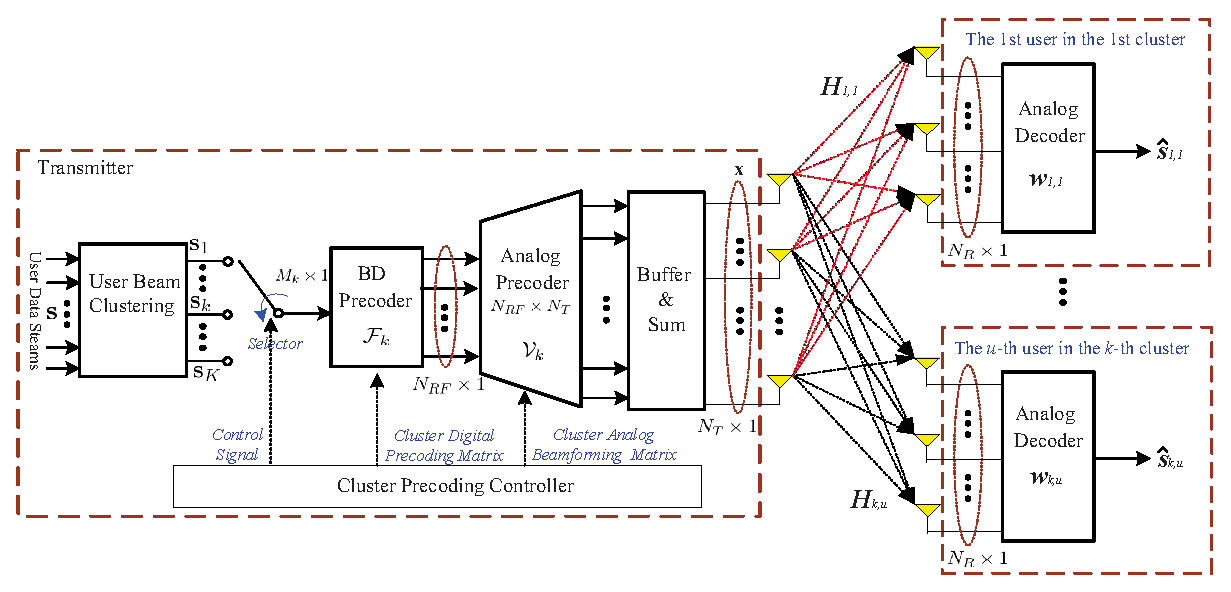
\includegraphics[height=2.8in,width=5.6in]{PPTFigure/BlockDiagonal.eps}
	\caption{Block diagram of the hybrid precoding system under consideration}\label{fig:BlockDiagram}
%	\parbox{6.5cm}{\small \hspace{1.5cm} }
\end{minipage}
\end{figure*}

\section{introduction}
To meet the ever-increasing demand of higher user data rates, it is envisioned that the next-generation cellular systems will be equipped with massive antenna arrays \cite{boccardi2014five}. Capitalizing on the large number of antennas at the base-station (BS), beam division multiple access (BDMA) has recently been proposed to transmit multiple users' data-streams via different beams \cite{sun2015beam, Jiang2018}. In contrast to the more conventional multiple access schemes such as Code Division Multiple Access (CDMA) or Orthogonal Frequency Multiple Division Access (OFDMA) that multiplex users in code, time and frequency domains, BDMA separates users in the beam space by transmitting data to different users in orthogonal beam directions. In \cite{sun2015beam}, BDMA was first proposed to decompose the multiuser multiple-input multiple-output (MU-MIMO) system into multiple single-user MIMO channels by multiplexing multiple users' data onto non-overlapping beams. BDMA is particularly attractive in practice as beamforming is commonly implemented in the analog domain using low-cost phase shifters. More recently, joint user scheduling and beam selection for BDMA was formulated under the Lyapunov-drift optimization framework before the optimal user-beam scheduling policy was derived in a closed form \cite{Jiang2018}. However, the assumption of non-overlapping orthogonal beams is hard to be satisfied, which handicaps the analog-only BDMA applications. In contrast, fully digital precoding has been developed to eliminate the inter-user interference through digital signal processing techniques. However, fully digital precoding requires a dedicated radio frequency (RF) chain per each antenna\cite{bogale2014beamforming}.

Despite its many performance advantages, such a fully digital precoding design is prohibitively expensive for massive MIMO systems. To cope with the obstacle, hybrid digital and analog beamforming has been developed for massive MIMO transmissions by dividing the procoding process into two steps, namely analog and digital precoding \cite{han2015large, el2014spatially}. More specifically, the transmitted signals are first precoded digitally using a smaller number of RF chains followed by the analog precoding implemented with a much larger number of phase shifters. As a result, the hybrid analog-digital precoding architecture requires significantly less RF chains as compared to the fully digital precoding. To further reduce the computational complexity, the notion of \textit{block diagonal} (BD) precoding was first introduced \cite{spencer2004zero}. By converting the inverse of a large matrix into the inverse of  multiple much smaller matrices, the BD precoding can be efficiently implemented with only marginal or no performance degradation as compared to the full digital precoding\cite{spencer2004zero}. The BD design has been recently extended to the hybrid precoding \cite{ni2016hybrid, liu2014phase}. However, most existing hybrid BD precoding schemes were developed based on a crucial assumption, i.e. the number of RF chains must be no less than the total number of data streams to be transmitted. Some pioneering proposals have been explored to relax this constraint by exploiting the state-of-the-art fast-speed phase shifters and switches that are capable of changing their states symbol by symbol \cite{garcia2017mimo}. However, \cite{garcia2017mimo} requires users to recover their symbols via the compressive sensing technique, which makes the scheme in \cite{garcia2017mimo} not suitable for low-complexity receivers.

In this paper, we consider a multiuser massive MIMO downlink system in which the transmitter sends more data streams with less RF chains by exploiting the hybrid BD precoding architecture built upon the state-of-the-art fast-speed phase shifters and switches. Unlike \cite{garcia2017mimo}, we consider low-complexity receivers that only perform analog beamforming. Our contributions are summarized as follows:

\begin{itemize}[leftmargin=*]
\item To transmit more data streams with less RF chains, we propose a cluster-by-cluster hybrid precoding scheme that effectively decomposes a large digital precoding matrix into block diagonal matrices. More specifically, users are first divided into $K$ clusters before their signals are precoded in the digital and analog domains cluster by cluster. As a result, the minimum number of RF chains is constrained by the number of data streams in each cluster, in lieu of the total number of data streams in the system. After precoding, all precoded cluster signals are summed together before transmission.\
\item While analog beamforming in our proposed precoding scheme can suppress much inter-cluster interference, the residual inter-cluster interference as well as the intra-cluster interference have to be removed via digital precoding. In this work, we derive two distinguishing digital precoders, namely the zero-forcing and the signal-to-leakage-and-noise (SLNR)-based precoders. Both precoders show good performance in simulation.
\item Most existing hybrid BD precoding schemes send multiple data streams to each user. As a result, it is a natural design to digitally precode each user's data streams while using analog beamforming to separate users. In sharp contrast, we consider the scenario where each scheduled user has only one data stream. Then, user clustering plays an important role in determining the system performance, therefore, we develop a greedy clustering algorithm to further improve the sum-rate of the whole hbrid BD precoding system.
\end{itemize}

%The structure of this paper is arranged as follows: the massive MIMO system with asynchronous hybrid BD precoding is introduced in Section II; the design of transmit digital/analog precoding matrix and receive analog beamforming vectors are elaborated in Section III; The user clustering algorithm is detailed in Section IV whereas the simulation results are shown in Section V; and finally we conclude the paper in Section VI

\underline{Notation}: Vectors and matrices are denoted by boldface letters. $\bm{I}_N$ denotes the identity matrix with size $N\times N$. ${\bm A}^T$ and ${\bm A}^H$ denote transpose and conjugate transpose of ${\bm A}$, respectively. $\bm{A}^\dagger$ being the pseudo inverse of $\bm{A}$ while $\|\bm{A}\|_0$, $\|\bm{A}\| $ and $|\bm{A}|$ stand for $0$ norm, the Frobenius norm and determinant of ${\bm A}$, respectively. $\bm{A}(i,j)$ denotes the $i$ row, $j$ column element of ${\bm A}$; $|\mathcal{I}|$ is the cardinality of the enclosed set ${\cal I}$; Finally, $\mathbb{E}[\cdot] $ denotes the expectation of a random variable.

\section{system model}
We consider a MU-MIMO downlink system as shown in \figurename{\ref{fig:BlockDiagram} in which $N_U$ out of $N_{tot}$ users are scheduled for service. The base station (BS) equipped with $N_{RF}$ RF chains and $N_T$ antennas transmits $N_U$ data streams to $N_U$ receivers with $N_R$ receive antennas. We assume only one data stream is designated to each scheduled receiver. Denoted by ${\bm s}(n)$ the $n$-th block of $N_U$ data to be transmitted, ${\bm s}(n)$ has unit power with $\mathbb{E}\left[\bm{ss}^H\right]=\frac{1}{N_U}\bm{I}_{N_U}$. In the sequel, we concentrate on a single block and omit the temporal index $n$ for notational simplicity.

\subsection{Transmitter}
In our proposed cluster-by-cluster BD digital precoding scheme, the $N_U$ users are first divided into $K$ clusters with the cluster size being $0< M_k\leq N_U$ for $k=1,2,\cdots,K$. It is clear that $\displaystyle\sum_{k=1}^{K} M_k = N_U$. Accordingly, the data streams $\bm{s}$ can be rewritten in clusters as:
\begin{equation}
\bm{s} = \left[{\mathbf{s}}_1^T, {\mathbf{s}}_2^T,\cdots, \mathbf{s}_{K}^T\right]^T,
\end{equation}
where $\mathbf{s}_k\in \mathcal{C}^{M_k\times 1}$ is the data vector transmitted to the users in the $k$-th cluster and modeled as:
\begin{equation}
\mathbf{s}_k = \left[s_{k,1}, s_{k,2},\cdots, s_{k,M_k}\right]^T,
\end{equation}
with $s_{k,u}$ being the data transmitted to the $u$-th user in $k$-th cluster for $u=1,2,\cdots,M_k$.

Next, we start with modeling the digital precoding process. Denote by $\bm{\mathcal{F}}_k$ of $N_{RF}\times M_k$ the digital precoder for the $k$-th cluster for $k=1,2,\cdots, K$, $\bm{\mathcal{F}}_k$ can be written as:
\begin{equation}
\bm{\mathcal{F}}_k = \left[\bm{f}_{k,1},\bm{f}_{k,2},\cdots,\bm{f}_{k,M_k}\right],
\end{equation}
where $\bm{f}_{k,u}$ represents the digital precoding vector for the $u$-th user in $k$-th cluster. Thus, the overall digital precoding matrix can be modeled as a block diagonal matrix as follows:
\begin{equation}
\bm{F} =
\begin{bmatrix}
\bm{\mathcal{F}}_1&\cdots & \bm{0}&\bm{0}\\
\vdots & \bm{\mathcal{F}}_2 & \vdots&\vdots \\
\bm{0}&\cdots&\ddots &\bm{0}\\
\bm{0}&\cdots & \bm{0}&\bm{\mathcal{F}}_K
\end{bmatrix}.\label{eq:DigPrecoderF}
\end{equation}
It is worth noting that inverting a BD matrix is less computationally
expensive than a non-BD matrix of the same dimension. Therefore, the BD structure of $\bm{F}$ in Eq.~(\ref{eq:DigPrecoderF}) can potentially lead to reduced computational complexity.

Similarly, we model the corresponding analog precoder in clusters as
\begin{equation}
	\bm{V} = \left[\bm{\mathcal{V}}_1, \bm{\mathcal{V}}_2,\cdots, \bm{\mathcal{V}}_{K}\right], \end{equation}
where $\bm{\mathcal{V}}_k$ of $N_T\times N_{RF}$, the analog precoder for the $k$-th cluster for $k=1,2,\cdots, K$, is given by:
\begin{equation}
\bm{\mathcal{V}}_k = \left[\bm{v}_{k,1},\bm{v}_{k,2},\cdots,\bm{v}_{k,M_k}\right].
\end{equation}
with $\bm{v}_{k,u}$ being the analog beamforming vector for the $u$-th user in $k$-th cluster.

Finally, the resulting hybrid precoded signal $\bm x \in\mathbb{C}^{N_T\times 1}$ is transmitted to all $N_U$ users.
\begin{equation}{\label{eq:transx}}
{\bm x} =  \bm{V}\cdot \bm{F}\cdot\bm{s} =\sum_{k=1}^K \bm{\mathcal{V}}_k \bm{\mathcal{F}}_k \mathbf{s}_k.
\end{equation}


\subsection{Channel Model}

Denote by $\bm{H}_{k,u}\in\mathbb{C}^{N_R\times N_T}$, the \textit{single-path} MIMO channel matrix between the transmitter and the $u$-th receiver in the $k$-th cluster is modeled using the Saleh-Valenzuela model\cite{rappaport2014millimeter}.
\begin{equation}{\label{eq:Hu}}
\bm{H}_{k,u} = \sqrt{N_{T}N_{R}}\alpha_{k,u}\cdot \bm{a}_{R}(\phi^r_{k,u},\theta^r_{k,u}) \cdot\bm{a}_{T}^{H}(\phi^t_{k,u},\theta^t_{k,u}),
\end{equation}
where $\alpha_{k,u}$, $\theta^r_{k,u}/\phi^r_{k,u}$ and $\theta^t_{k,u}/\phi^t_{k,u}$ are the complex path gain, azimuth/elevation angles of arrival(AoA) and azimuth/elevation angles of departure(AoD) of the $u$-th user in the $k$-th cluster, respectively. Furthermore, $\bm{a}(\phi,\theta)$ is the array response vector. For an uniform planar array (UPA) of size $P\times Q$ considered in this work, the array response vector is given by \cite{alkhateeb2014channel}
\begin{flalign}\label{eq:UPAvec1}
\bm{a}(\phi,\theta) =&\frac{1}{\sqrt{N_T}}\left[1,  e^{j\kappa d(\sin\phi \sin\theta +\cos\theta)},  e^{j2\kappa d(\sin\phi \sin\theta +\cos\theta)}, \right. &&\nonumber\\
&\left. \cdots, e^{j\kappa d\left((P-1)\sin\phi \sin\theta +(Q-1)\cos\theta\right)}\right]^T,&&
\end{flalign}
where $\kappa =\frac{2\pi}{\lambda}$ is the wavenumber and $d$ is the distance between two adjacent antennas. Even though in this paper single-path channel model is considered, it should be noted that the efficacy of our proposed transmission scheme in the sequel still holds for multi-path scenarios.

%In this work, we assume that each scatter only contributes one single propagation path, i.e. $L_{k,u}=1$, which is a common assumption in the literatures.

\subsection{Receiver}

The signal received by the $u$-th user in the $k$-th cluster is given by
\begin{eqnarray}{\label{eq:rewrite}}
{\bm y}_{k,u} &=&\underbrace{\bm{H}_{k,u} \bm{\mathcal{V}}_k\bm{f}_{k,u}{s}_{k,u}}_\text{Desired Signal}+\underbrace{\bm{H}_{k,u} \bm{\mathcal{V}}_k\sum_{\substack{i=1 \\ i\neq u}}^{M_K}\bm{f}_{k,i}s_{k,i}}_\text{Intra-cluster Interference} \nonumber\\
&+& \underbrace{\bm{H}_{k,u}\sum_{\substack{j=1\\j\neq k}}^{K}\bm{\mathcal{V}}_j\bm{\mathcal{F}}_j\bm{s}_j}_\text{Inter-cluster Interference}+ \underbrace{\bm{n}_{k,u}}_\text{Noise}
\end{eqnarray}
where $\bm{n}_u$ is complex additive white Gaussian noise with zero mean and variance equal to $\sigma^2$.

Assuming the receivers are all low-cost terminals that perform analog beamforming only in decoding, the decoded signal by the $u$-th user in $k$-th cluster denoted by $\hat{s}_{k,u}$ is given by :
\begin{equation}{\label{eq:hats}}
\hat{s}_{k,u} = \bm{w}_{k,u}^H \bm{H}_{k,u} \bm{\mathcal{V}}_k \bm{f}_{k,u} s_{k,u} + \bm{w}_{k,u}^H \bm{\tilde{n}}_{k,u},
\end{equation}
where ${\bm w}_{k,u}$ of length $N_R$ is the analog beamforming vector employed by the $u$-th receiver with the power constraint of $|\bm{w}_{k,u}|^2=1$ and
\begin{equation}\label{Eq:ntilde}
\bm{\tilde{n}}_{k,u}=\bm{H}_{k,u} \bm{\mathcal{V}}_k\sum_{\substack{i=1 \\ i\neq u}}^{M_K}\bm{f}_{ki}s_{ki} + \bm{H}_{k,u}\sum_{\substack{j=1\\j\neq k}}^{K}\bm{\mathcal{V}}_j\bm{\mathcal{F}}_j\bm{s}_j+  \underbrace{\bm{w}_{k,u}^H \bm{n}_{k,u}}_\text{Noise}.
\end{equation}
Note that the first term in Eq.~(\ref{eq:hats}) stands for the desired signal while the second term is the sum of its own receiver noise and interference from intra-cluster users and other clusters' users.

\subsection{Cluster-by-Cluster(CbC) hybrid precoding}
For notational simplicity, we denote by ${\bm{g}}^{(j)H}_{k,u}$ the effective analog beamforming gain vector observed by the $u$-th user in the $k$-th cluster from the $j$-th cluster for $j,k=1,2,\cdots,K$.
\begin{equation}\label{eq:def}
{\bm{g}}^{(j)H}_{k,u} = \bm{w}^H_{k,u} \bm{H}_{k,u} \bm{\mathcal{V}}_{j}.
\end{equation}

Assuming that the power allocated to each user is uniform, the signal-to-noise ratio can be represented as $\gamma = \frac{P}{\sigma^2N_U}$ where $P$ is the total power in transmitter and $\sigma^2$ is the noise power. Then channel capacity of the $u$-th user can be computed as
\begin{equation}\small\label{eq:convenR}
R_{k,u} = \log\left(1+\frac{\gamma|{\bm{g}}_{k,u}^{(k)H} \bm{f}_{k,u}|^2}{\gamma\displaystyle\sum_{\substack{i=1 \\ i\neq u}}^{M_k}\Big(|{\bm{g}}_{k,u}^{(k)H}\bm{f}_{ki}|^2+\displaystyle\sum_{\substack{j=1\\j\neq k}}^{K}\|\bm{g}_{k,u}^{(j)H}\bm{\mathcal{F}}_j\|^2\Big)+1}\right).
\end{equation}

Subsequently, the system sum-rate capacity can be computed as a function of $\bm{W}$, ${\bm V}$ and ${\bm F}$:
\begin{equation}
R_{tot}(\bm{W}, \bm{V}, \bm{F})=\sum_{k=1}^{K}\sum_{u=1}^{M_k}R_{k,u}.
\end{equation}

For conventional hybrid beamforming with sufficient RF chains, the digital beamforming vectors can be designed to eliminate inter-user interference, i.e.
{\color{red}\begin{equation}
 \displaystyle\sum_{\substack{i=1 \\ i\neq u}}^{M_k}\Big(|{\bm{g}}_{k,u}^{(k)H}\bm{f}_{ki}|^2+\displaystyle\sum_{\substack{j=1\\j\neq k}}^{K}\|\bm{g}_{k,u}^{(j)H}\bm{\mathcal{F}}_j\|^2\Big)={0}. 
\end{equation}
}
In contrast, since the proposed BD precoding scheme requires less RF chains, i.e. $N_{RF}\leq N_U$, it can only achieve interference-free asymptotically as $N_T$ grows large. Thus, the capacity of the proposed BD precoding is limited by the residual interference in the system. Given $K$ clusters, we can derive the optimal analog and block digital precoding matrices by
\begin{align}\label{eq:maxsumrate}
P_1: \quad&\max_{\bm W, \bm{V},\bm F, }\quad R_{tot}(\bm{W}, \bm{V}, \bm{F})\\ \nonumber
s.t. \quad&C_1: \|\bm{v}_{k,u}\|^2_2=1; \\
&C_2: \|\bm{w}_{k,u}\|^2_2=1;\nonumber\\
&C_3: \|\bm{\mathcal{V}}_k \bm{f}_{k,u}\|^2=1;\nonumber\\
&C_4: \bm{V} = [\bm{\mathcal{V}}_1, \bm{\mathcal{V}}_2, \cdots, \bm{\mathcal{V}}_K];\nonumber\\
&C_5: \bm{F} = \text{diag}(\bm{\mathcal{F}}_1, \bm{\mathcal{F}}_2, \cdots, \bm{\mathcal{F}}_{K});\nonumber\\
&C_6: \max \{M_k\}_{k=1}^K \leq N_{RF};\nonumber
\end{align}
where $k=1,2,\cdots,K$ and $u = 1, 2, \cdots, M_k$ in $C_1$, $C_2$ and $C_3$. $C_1$ and $C_2$ confine all analog beamforming vectors to phase-only style and $C_3$ ensures the power applied on each signal by transmit precoders is of unit power. $C_4$ defines the structure of digital prcoder, and $C_5$ specifics the structure of BD digital precoding matrix. Finally,  $C_6$ depicts that the maximal data streams in each cluster is upper bounded by the number RF chains. 
%$C_6$ is the introduced switch matrix which can change the sequence of transmitted data streams. $\bm{t}_{i}$ and $\bm{t}_{j}$ are the row and column vectors of $\bm{T}$, respectively.

The problem $P_1$ is challenging due to its non-convex and combinatorial nature. Thus, it is analytically intractable to derive the optimal solution. Instead, we consider a two-stage suboptimal solution: In the first stage, we focus on the analog  and digital precoders design to minimize the inter-user interference ; After fixing the analog and digital precoders, we leverage user clustering to further improve system sum-rate in the second stage.

\section{proposed block hybrid beamforming for RF chains reduction}
In this section, we will first optimize the analog precoder before deriving two digital precoders, namely the block zero-forcing (BZF) and block signal-to-leakage-and-noise ratio (SLNR) maximization (BSM) precoders. When designing the digital and analog precoders, we assume the user clustering is given. That is to say we firstly solve the precoder optimization problem for a particular user clustering, and then handle the user clustering algorithm, knowing the precoders design. Even though the optimization problems in these two stages are all highly non-convex, we attempt at closed-form solutions for precoder design and low complexity solution for user clustering algorithm.

\subsection{Analog Beamforming Design}\label{analog}
In this subsection, we first focus on the analog beamforming design on both transmitter and receiver sides. According to the theory for infinite antenna theory, \textit{i.e.} as the number of transmit antennas goes to infinity, distinct array response vectors are asymptotically orthogonal, we have
\begin{equation}\label{Eq:assumption}
\lim_{N\rightarrow +\infty} \bm{a}_{T}^{H}(\phi^t_{k,u},\theta^t_{k,u}) \cdot\bm{a}_{T}(\phi^t_{\ell,v},\theta^t_{\ell,v})=\delta(k-\ell)\delta(u-v).
\end{equation}

Hence, to orthogonalize transmitted signals,  the transmit analog beamforming vector for user $u$ in cluster $k$ is designed as
\begin{equation}
\bm{v}_{k,u}=\bm{a}_{T}^{H}(\phi^t_{k,u},\theta^t_{k,u}),
\label{eq:vku}
\end{equation}
so that we expect the inter-user interference can be completely eliminated. Now, the equivalent channel from the transmitter to user $u$ in cluster $k$ is $\bm{H}_{k,u}\bm{v}_{k,u}=\sqrt{N_{T}N_{R}}\alpha_{k,u}\cdot \bm{a}_{R}(\phi^r_{k,u},\theta^r_{k,u})$ and the equivalent channels to other users are all equal to zero vectors. On the receiver side, we use maximum ratio combing (MRC) to design the analog beamforming vector \textit{i.e.}
\begin{equation}
\bm{w}_{k,u}=\bm{a}_{R}^{H}(\phi^r_{k,u},\theta^r_{k,u}),\\
\label{eq:wku}
\end{equation}

In practice, the number of transmitter antenna is finite, which means after transmit analog beamforming, the residual inter-user interference inherently exists. Thereby we need digital precoders to further suppress these interferences.

\subsection{Digital Precoder Design}\label{digital}
Ideally the digital precoder can be solved by the optimization problem $P1$ given analog design by Eq.\eqref{eq:vku} and Eq.\eqref{eq:wku}:
%\begin{align}\label{eq:digital}
%P_2: \quad&\max_{\bm F}\quad \sum_{k=1}^{K} R_{avg}(\bm{\mathcal{F}}_k)\\ \nonumber
%s.t. \quad &C_1: \|\bm{Vf}_u\|^2=1;\nonumber\\
%&C_2: \bm{F} = \text{diag}(\bm{\mathcal{F}}_1, \bm{\mathcal{F}}_2, \cdots, \bm{\mathcal{F}}_{K});\nonumber\\
%&C_3: \max \{M_k\}_{k=1}^K \leq N_{RF};\nonumber
%\end{align}
However, due to the non-complexity of Eq. \eqref{eq:convenR}, we failed to find the optimal closed-form solution of $\bm F$. Nevertheless, we provide two intuitive approaches that lead to high sum-rate.

\subsubsection{Blcok Zero Forcing (BZF)}
For a given number of users $K>N_{RF}$, the digital precoder is shaped by a block diagonal matrix as aforementioned. We firstly design the digital precoder for each block as the inverse of the effective channel of the block. Specifically, we have
\begin{equation}
\bm{\mathcal{F}}^{BZF}_{k} = \bm{\mathcal{G}}_k^H (\bm{\mathcal{G}}_k \bm{\mathcal{G}}_k^H)^{-1}
\end{equation}
with $N_{RF}\geq M_k$, where $\bm{\mathcal{G}}_k = [\bm{g}^{(k)}_{k,1}, \bm{g}^{(k)}_{k,2},\cdots,\bm{g}^{(k)}_{k,M_k}]^H$.

To satisfy the power constraint $C_3$ in $P_1$, power normalization is performed on each ${\bm f}_{k,u}$ derived from $\bm{\mathcal{F}}^{BZF}_{k}=\left[\bm{f}^{BZF}_{k,1},\bm{f}^{BZF}_{k,2},\cdots,\bm{f}^{BZF}_{k,M_k}\right]$ as
\begin{equation}\label{eq:ZFU-HBF2}
\bm{\bar{f}}^{BZF}_{k,u} = \frac{\bm{f}^{BZF}_{k,u}}{\|\bm{V}\cdot\bm{f}^{BZF}_{k,u}\|}.
\end{equation}

For a special case $K=1$, this problem can be simply solved by conventional zero-forcing.

%Compared to conventional digital precoding, the only difference is that the data streams are processed cluster-by-cluster such that the number of considered users is reduced from $N_U$ to $M_k$ for $k$-th cluster. Thus, the minimal number of required RF chains is then reduce to $N_{RF} = \max \{M_k\}_{k=1}^K$.

\subsubsection{Block SLNR Maximization(BSM)}
Although the BZF has good performance as shown in the simulation results, it requires to acknowledge all the channel information for each user.
The conventional SLNR maximization(SM) is considered as a criterion to reduce co-channel interference(CCI) and noise.  For the $u$-th user in cluster $k$, the received power of desired data streams can be expressed as
\begin{equation}
S_{k,u} = \gamma\left|\bm{g}_{k,u}^{(k)H}  \bm{f}^{BSM}_{k,u}\right|^2.
\end{equation}
In the meanwhile, the power leaked to other users is
\begin{align}
L_{k,u} = &\gamma\left(\sum_{\substack{j=1\\j\neq k}}^{K}\sum_{i=1}^{M_j}\left|\bm{g}_{j,i}^{(k)H} \bm{f}^{BSM}_{k,u}\right|^2+ \sum_{\substack{t=1\\t\neq u}}^{M_k}\left|\bm{g}_{k,t}^{(k)H} \bm{f}^{BSM}_{k,u}\right|^2\right).
\end{align}
Therefore, in contrast with the SINR expression in Eq.\eqref{eq:convenR}, the SLNR for the $u$-th user in $k$-th cluster can be expressed as


\begin{equation}\label{eq:slnr}
\phi_{k,u} = \frac{\left|\bm{g}_{k,u}^{(k)H}  \bm{f}^{BSM}_{k,u}\right|^2}{\displaystyle\sum_{\substack{j=1\\j\neq k}}^{K}\displaystyle\sum_{i=1}^{M_j}\left|\bm{g}_{j,i}^{(k)H} \bm{f}^{BSM}_{k,u}\right|^2+ \displaystyle\sum_{\substack{t=1\\t\neq u}}^{M_k}\left|\bm{g}_{k,t}^{(k)H} \bm{f}^{BSM}_{k,u}\right|^2+{1\over \gamma}}.
\end{equation}

Preceding studies (e.g.\cite{wang2012statistical}) show that the digital precoder maximizing SLNR $\phi_{k,u}$ is tractable i.e.,
\begin{equation}\small
\bm{f}^{BSM}_{k,u} = 
\mathbf{u}_{max}\left( \left(\frac{1}{\gamma}\bm{I}+\bm{Q}_{k,u} \right)^{-1}{\bm{g}}_{k,u}^{(k)}{\bm{g}}_{k,u}^{(k)H}\right),
\end{equation}
where $\bm{Q}_{k,u}$ is the covariance of the leakage given arisen from $u$-th user in $k$-th cluster:

\begin{equation}
\bm{Q}_{k,u}=\displaystyle\sum_{\substack{j=1\\j\neq k}}^{K}\displaystyle\sum_{i=1}^{M_j}\bm{g}_{j,i}^{(k)}\bm{g}_{j,i}^{(k)H} + \displaystyle\sum_{\substack{t=1\\t\neq u}}^{M_k}\bm{g}_{k,t}^{(k)} \bm{g}_{k,t}^{(k)H}.
\end{equation}

Still, we need to normalize the digital precoder as with Eq.\eqref{eq:ZFU-HBF2}. Note that after obtaining the digital precoders, we must align all of them in clusters to get the entire BD digital precoding matrix in Eq.\eqref{eq:DigPrecoderF}.

Here, which users should be gathered into a cluster becomes an important question that surely would steer the performance of the whole multi-user system. In what follows, a heuristic user clustering algorithm is provided.
\subsection{User Clustering}
In this subsection, we propose a user clustering algorithm designated to BZF precoder, which also shows considerably good performance for BSM. Recalling that BZF digital precoder can eliminate the intra-cluster interference, we will cluster users to minimize the inter-cluster interference. 

Ignoring the intra-cluster interference, we approximate the capacity of $u$-th user in $k$-th cluster by
\begin{align}\label{capacity}\small
\tilde{R}_{k,u} \approx \log\left(1+\frac{\|\bm{w}^H_{k,u} \bm{H}_{k,u} \bm{\mathcal{V}}_{k}\|^2}{\displaystyle\sum_{j=1,j\neq k}^{K}M_j\|{\bm{w}}^H_{k,u} \bm{H}_{k,u} {\bm{\mathcal{V}}}_j\|^2+{1\over \gamma}}\right).
\end{align}
The approximation is based on that each channel is independently and identically Rayleigh distributed, so that we can have $\bm{\mathcal{F}}^{BZF}_{k} = \bm{\mathcal{G}}_k^H (\bm{\mathcal{G}}_k \bm{\mathcal{G}}_k^H)^{-1}\approx \mathbf{I}_{M_k}$.

We propose a Greedy Clustering Algorithm~\ref{beam_cluster} by exchanging the index of data stream. In this greedy clustering algorithm,  the users are clustered to different centers by maximizing the sum-rate capacity. The rows indexed from 20 to 22 in Algorithm~\ref{beam_cluster} take into account the constraint on the number of RF chains required for each cluster.
%From Section \ref{analog}, we know that the analog precoder $\bm{\mathcal{V}}_k$ is a function of $\bm{H}_{k,u}$. Thus we introduce a switch matrix $\bm{T}$ that can change the index of data stream.

%\begin{align}
%P_2: \{\{\bm{\mathcal{V}}^*_k\}_{k=1}^{K}, \bm{T}^*\}=& \argmax \sum_{k=1}^{K}\sum_{u=1}^{M_k} \tilde{R}_{k,u}\left(\bm{\tilde{\mathcal{V}}}_k, \bm{H}_{k,u}(\bm{\tilde{T}})\right)\\
%s.t. &\quad\max\{M_k\}_{k=1}^K \leq N_{RF}.\nonumber
%\end{align}

%In this problem, the digital precoder $\bm{\mathcal{F}}_k$ of $k$-th cluster can be solved by the proposed approaches in section \ref{digital} after obtaining the analog precoder of clustered users. To realize clustering, $\bm{T}$ is a switch matrix that can exchange the vectors of original analog precoder.
%
%Considering the np-hardness of $P_3$, $\bm{T}$ is difficult to be analytically solved. Rather than directly optimizing $\bm{T}$ by exhaustively searching all possible combinations, we propose a greedy clustering algorithm in Algorithm~\ref{beam_cluster} to cluster users. 

\begin{algorithm}[h] 		
	\caption{Greedy clustering algorithm for block hybrid beamforming system}
	\label{beam_cluster}
	\begin{algorithmic}[1]
		\REQUIRE  \quad
		\STATE	Denote all user index as $\mathcal{X}$ \\
		\STATE  Initialize the user index set in $k$-th cluster as $\mathcal{I}_k=\emptyset$, $k=1,2,\cdots, K$\\
		\STATE 	Initialize the user index with cluster index set : $\bm{\mathcal{I}}=\emptyset$
		\STATE  Cluster index set: $\mathcal{K}$\\
		\ENSURE   	
		\STATE Assign a user index with largest channel gain $x^*$ corresponding to ${\mathcal I}_1$, {\em i.e.} $\mathcal{I}_1 \leftarrow  (1, x^*)$,  $\bm{\mathcal{I}} \leftarrow \mathcal{I}_1$ and ${\mathcal X}\setminus x^*$,
		\WHILE{$\mathcal{X}$ is not empty}
		\FOR{$k$ in $\mathcal{K}$}
		\FOR{$x$ in ${\mathcal{X}}$}
		\STATE  Update the auxiliary set $\bar{{\mathcal{I}}}_k$ by adding $(k,x)$ to $\mathcal{I}_k$
		\STATE  Update the auxiliary set $\bar{\bm{\mathcal{I}}}$ by adding $\bar{\mathcal{I}}_k$ to ${\bm{\mathcal{I}}}$
		\STATE Calculate the sum-rate capacity by Eq. \eqref{capacity} $${R}(k,x)= \sum_{(j,u)\in \bar{\bm{\mathcal{I}}}} \tilde{R}_{j,u}$$
		\ENDFOR
		\STATE Find the user index $(k^*,x^*)$ with maximum $R(k,x)$
		\STATE Update $\mathcal{I}_{k}\leftarrow (k^*, x^*)$, $\bm{\mathcal{I}}\leftarrow \mathcal{I}_k$ and  ${\cal X}\setminus x^*$
		\ENDFOR
		\IF{\textit{cardinality}$(\mathcal{I}_k)== N_{RF}$}
		\STATE ${\mathcal{K}} \setminus k$
		\ENDIF
		\ENDWHILE
	\end{algorithmic}
\end{algorithm}

\section{simulation results}
In this section, we use computer simulation to compare the performance of sum-rate capacity for RF chains-reduction algorithm. Unless specified otherwise, we consider a transmitter equipped with an $12\times 12$ UPA ({\em i.e.} $N_T=144$) and $N_U=16$ users each equipped with a $8\times 8$ UPA ({\em i.e.} $N_R=64$). The channels are multi-path with the azimuth AoAs/AoDs being uniformly distributed over $[0, 2\pi]$ and the elevation AoAs/AoDs being uniformly distributed in $[-\pi/2, \pi/2]$, respectively. For each computer experiment, we compute the average over 500 realizations.

We firstly compare the two proposed digital precoding approaches with conventional algorithm. As shown in Fig.~\ref{fig:MultiuserGain}, the dash line ``ZF'' is the conventional zero-forcing precoding system where $2\times 8$ RF chains are required to serve $2\times 8$ users.  The BDMA is the analog-only precoding system. For the sake of fairness, the sum-rate capacities of dash lines are divided by 2. The solid lines represent the proposed RF chains reduction hybrid beamforming systems where only 8 RF chains are used to serve 16 users using CbC. The performance of block zero-forcing without clustering can be significantly increased by the proposed block zero-forcing (BZF) and block SLNR maximization (BSM) with clustering. The performances of BZF and BSM are very similar.

\begin{figure}[ht]
	\begin{center}
		\includegraphics[width=3.2in,height=2.5in]{Figure/comp1path.eps}
		\caption{Sum-rate capacity comparison with different algorithm.}\label{fig:MultiuserGain}
	\end{center}
\end{figure}

\begin{figure}[ht]
	\begin{center}
		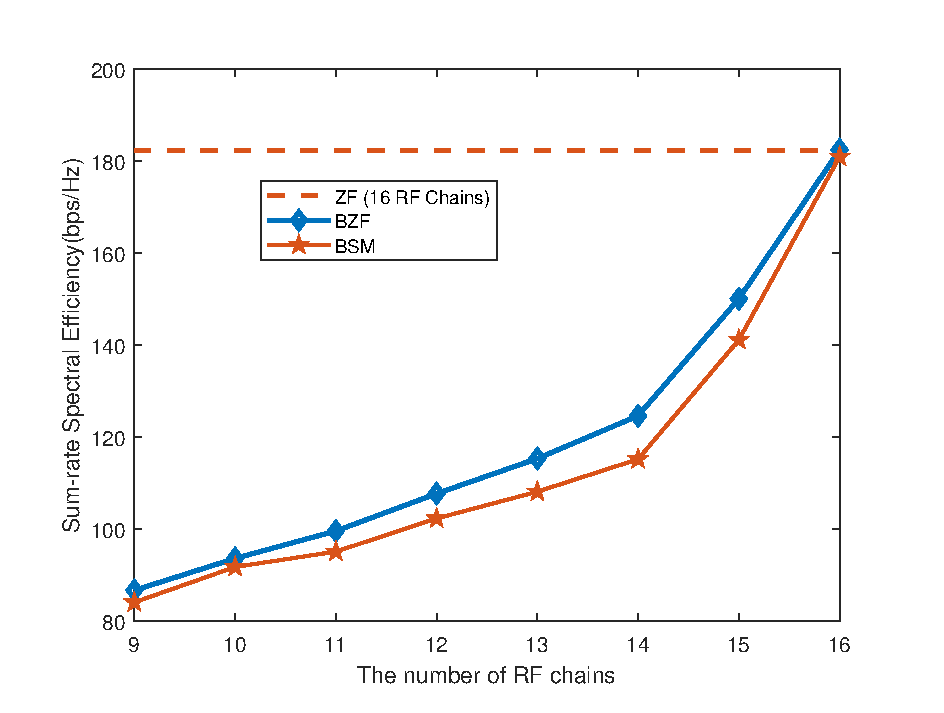
\includegraphics[width=3.2in,height=2.6in]{Figure/differentRF1path.eps}
		\caption{Different number of RF chains.}\label{fig:RFchains}
	\end{center}
\end{figure}
In Fig.~\ref{fig:RFchains}, we can see that the sum-rate capacity will increase as more RF chains added. The upper bound is the zero-forcing precoding system with 16 RF chains for 16 users. The conventional ZF is the hybrid precoding system with 8 RF chains for 8 users.

\begin{figure}[ht]
	\begin{center}
		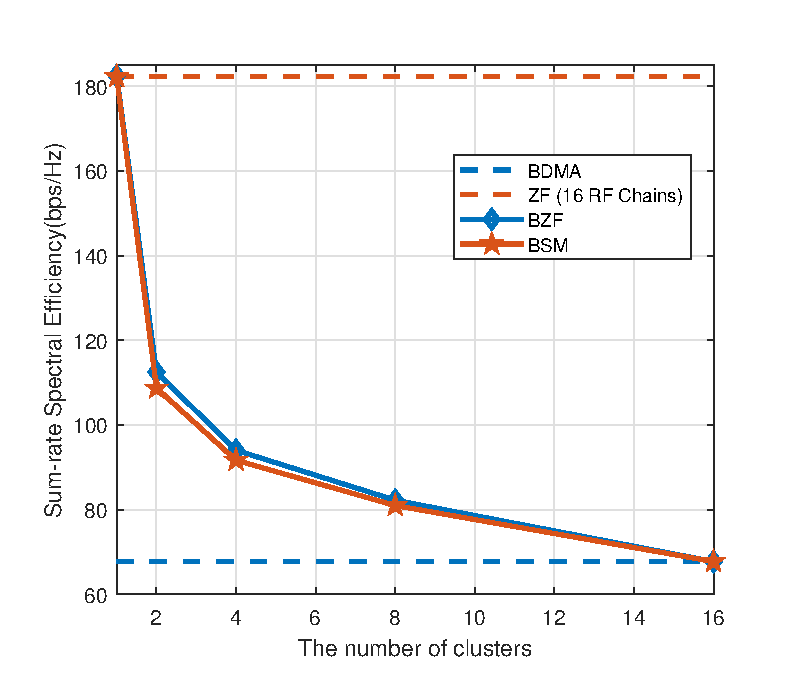
\includegraphics[width=3.2in,height=2.6in]{Figure/differentK1path.eps}
		\caption{The comparison for different number of clusters.}\label{fig:differentK}
	\end{center}
\end{figure}

\begin{figure}[ht]
	\begin{center}
		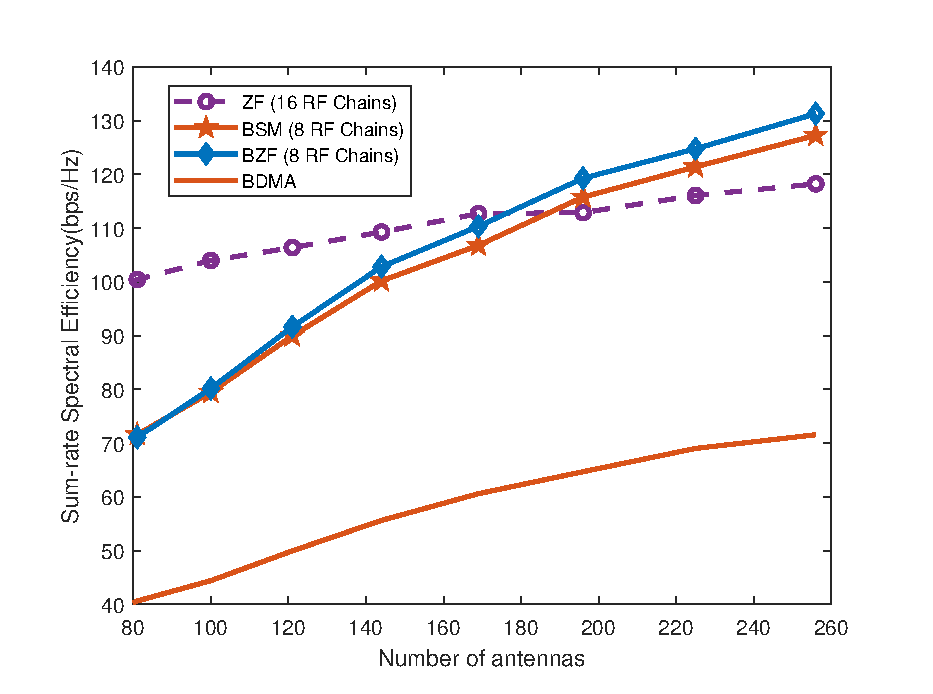
\includegraphics[width=3.2in,height=2.6in]{Figure/antenna1path.eps}
		\caption{The sum-rate capacity for different number of antennas in transmitter.}\label{fig:CDF}
	\end{center}
\end{figure}


The Fig. \ref{fig:differentK} shows that the BZF and BSM are lower bounded by the BDMA and upper bounded by conventional zero-forcing. The system is converted as a conventional hybrid beamforming system when the number of RF chains is not less than data streams. For 16 clusters system, the system is simplified as an analog-only  beamforming system.

Finally, the performance for different systems with increasing number of antennas is shown in Fig. \ref{fig:CDF}. By varying the number of antennas, we investigate the sum-rate capacity improvement. The capacity of BZF and BSM will significantly increase as the increment of antennas. The reason is that the residual interference from Eq. \eqref{Eq:assumption} will be reduced for more antennas.

\section{Conclusion}
In this work, we have developed block clustering precoding scheme for mmWave massive MIMO systems by jointly performing hybrid analog-digital precoding and user-beam clustering. First, we have modeled the block hybrid precoder design to reduce the required RF chains by processing the data streams cluster-by-cluster and the analog precoder can be solved by greedily maximizing the sum-SIR. Furthermore, two approaches are proposed, namely BZF and BSM, to obtain the digital precoder. Simulation results have confirmed that the proposed block clustering precoding scheme can achieve better sum-rate capacity with less RF chains compared to the conventional hybrid precoding scheme. The two approaches BZF and BSM can be considered to have the equivalent performance.


\bibliography{BDMAref}
\bibliographystyle{IEEEtran}


% references section

\end{document}


